\documentclass[12pt,a4paper,ngerman]{report}
\usepackage{babel}
%\usepackage{natbib}
\usepackage{url}
%\usepackage[left=2cm, right=1.5cm, top=2cm, bottom=2cm]{geometry}
%\usepackage[ansinew]{inputenc}
\usepackage{amsmath}
\usepackage{nicefrac} % macht schöne Brüche mit querstrich mit \nicefrac{1}{2}
\usepackage{graphicx}
%\graphicspath{}
\usepackage{titlesec}% um chapterüberschriften anzupassen.
\titleformat{\chapter}{\normalfont\huge\bf}{\thechapter.}{20pt}{\huge\bf}
\usepackage{parskip}
\usepackage{fancyhdr}
\usepackage{amsfonts}
\usepackage{float}
\usepackage{caption}
\usepackage{subcaption} % for \begin{subfigure}
	
\usepackage{csquotes} % mit \enquote{blabla} tolle anfürungsstriche erstellen
%\usepackage{physics} %lässt mich \bra und \ket benuzen %im konflict mit siunitx

\usepackage{pgfplots} %für plots
\pgfplotsset{compat=newest}

\usepackage{varioref} % macht mit \vref{} viel bessere referenzen
\usepackage{hyperref} % macht klickbare referenzen

\usepackage{xcolor, soul} %mit \hl{} kann man toll Sachen hervorheben.
\newcommand{\highlight}[1]{%
	\colorbox{yellow!50}{$\displaystyle#1$}} % mit \highlight{} kann man sogar in Gleichungen hervorheben

\usepackage{vmargin}
\usepackage[section]{placeins}
\usepackage{capt-of}
\usepackage{enumitem}
\usepackage{multirow}
\usepackage{blindtext}
\usepackage[version=4]{mhchem} % um Chemische Elementsymbole zu benutzen: \ce{H20}

\usepackage{pdfpages} % um PDFs einzufügen

%spread to latex:
\usepackage{booktabs, multirow} % for borders and merged ranges
\usepackage{changepage,threeparttable} % for wide tables

\providecommand{\e}[1]{\ensuremath{\cdot 10^{#1}}}
\providecommand{\fehlt}{\textcolor{red}{{ ¡Fehlt! }}}

\providecommand{\versuchstitel}{Perowskitsolarzellen} % Hier den Versuchstitel eintragen!

\usepackage{siunitx}
\sisetup{
	separate-uncertainty = true,
	%per-mode = fraction,
	%per-mode = symbol
}
\DeclareSIUnit\bar{bar}
\DeclareSIUnit\atomicmassunit{u}
\usepackage{isotope}


\setmarginsrb{3 cm}{2.5 cm}{3 cm}{2.5 cm}{1 cm}{1.5 cm}{1 cm}{1.5 cm}
\title{\versuchstitel}


\author{Frederik Uhlemann, Florian Adamczyk}
% Author
\date{\today}
% Date

\makeatletter
\let\thetitle\@title
\let\theauthor\@author
\let\thedate\@date
\makeatother

\pagestyle{fancy}
\fancyhf{}
\rhead{\theauthor}
\lhead{\versuchstitel}
\cfoot{\thepage}
%%%%%%%%%%%%%%%%%%%%%%%%%%%%%%%%%%%%%%%%%%%%
\begin{document}
		
	%%%%%%%%%%%%%%%%%%%%%%%%%%%%%%%%%%%%%%%%%%%%%%%%%%%%%%%%%%%%%%%%%%%%%%%%%%%%%%%%%%%%%%%%%
	
	\begin{titlepage}
		\centering
		\vspace*{0.5 cm}
		% \begin{large} Justus-Liebig-Universität\\ Gießen \end{large}
		
\includegraphics[width = 0.6 \textwidth]{JLU_Giessen-Logo}	%University Logo
		\\[2.0 cm]
		% \begin{center}    \textsc{\Large Justus - Liebig - Universität}\\{Giessen}\\[0.8cm]	\end{center}% University Name
		Versuch 7 des\\
		\textsc{\Large Fortgeschrittenen-Praktikums}\\ [0.3 cm]				% Course Code
		\rule{\linewidth}{0.2 mm} \\[0.4 cm]
		{ \huge \bfseries \thetitle}\\%%% TITEL HERE
		\rule{\linewidth}{0.2 mm}\\
		Versuchstermin 21.6.2024 \\
		~ \\
		[2.0 cm]
		
		
		\begin{minipage}{0.49\textwidth}
			\begin{flushleft}
				 \emph{Praktikumsbetreuer:}\\
				 M.Sc. Tim P. Schneider\\
				 %  Affiliation\\
				 \small{\href{mailto:tim.schneider@ap.physik.uni-giessen.de}{tim.schneider@ap.physik.uni-giessen.de}}
			\end{flushleft}
		\end{minipage}~
		\begin{minipage}{0.49\textwidth}
			\begin{flushright}
				\emph{Protokoll von:} \\
				
				\large{Frederik Uhlemann}\\
				\small{\href{mailto:frederik-vincent.uhlemann@physik.uni-giessen.de}{frederik-vincent.uhlemann@physik.uni-giessen.de}\\~\\
					%Matrikel Nr.: \:  \\[0.5cm]
					%\href{mailto:}{}
				}
				\large{Florian Adamczyk} \\
				\small{\href{mailto:florian.marius.adamczyk@physik.uni-giessen.de}{florian.marius.adamczyk@physik.uni-giessen.de}\\
					%Matrikel Nr.: \: 8105234}
			}
		\end{flushright}
	\end{minipage}
	
	\end{titlepage}
	
%%%%%%%%%%%%%%%%%%%%%%%%%%%%%%%%%%%%%%%%%%%%%%%%%%%%%%%%%%%%%%%%%%%%%%%%%%%%%%%%%%%%%%%%%
\setcounter{secnumdepth}{3}
\setcounter{tocdepth}{4}
\tableofcontents
%\newpage

%%%%%%%%%%%%%%%%%%%%%%%%%%%%%%%%%%%%%%%%%%%%%%%%%%%%%%%%%%%%%%%%%%%%%%%%%%%%%%%%%%%%%%%%%
%\renewcommand{\thesection}{\arabic{section}} %lässt in den subsections die erste zahl von darüberliegenden chapter weg.

%\pagebreak
	
%\setcounter{chapter}{-1}
\chapter*{Einleitung}\addcontentsline{toc}{chapter}{Einleitung}
	\fehlt

	% notiz an mich: mit "~ bewirke ich einen geschützten bindestrich an dem nicht getrennt werden darf.
	% nur eine ~ macht ein geschütztes (normales) Leerzeichen. \, macht ein halbes geschütztes Leerzeichen.

\chapter{Theorie}
	\section{Kenngrößen von Solarzellen}
	Als wird folgend auf die Grundsätzlichen Eigenschaften von Solarzellen eingegangen, damit die Eigenschaften der hergestellten Perowskitsolarzelle eingeordnet werden können.\\
	\begin{figure}[ht]
		\centering
		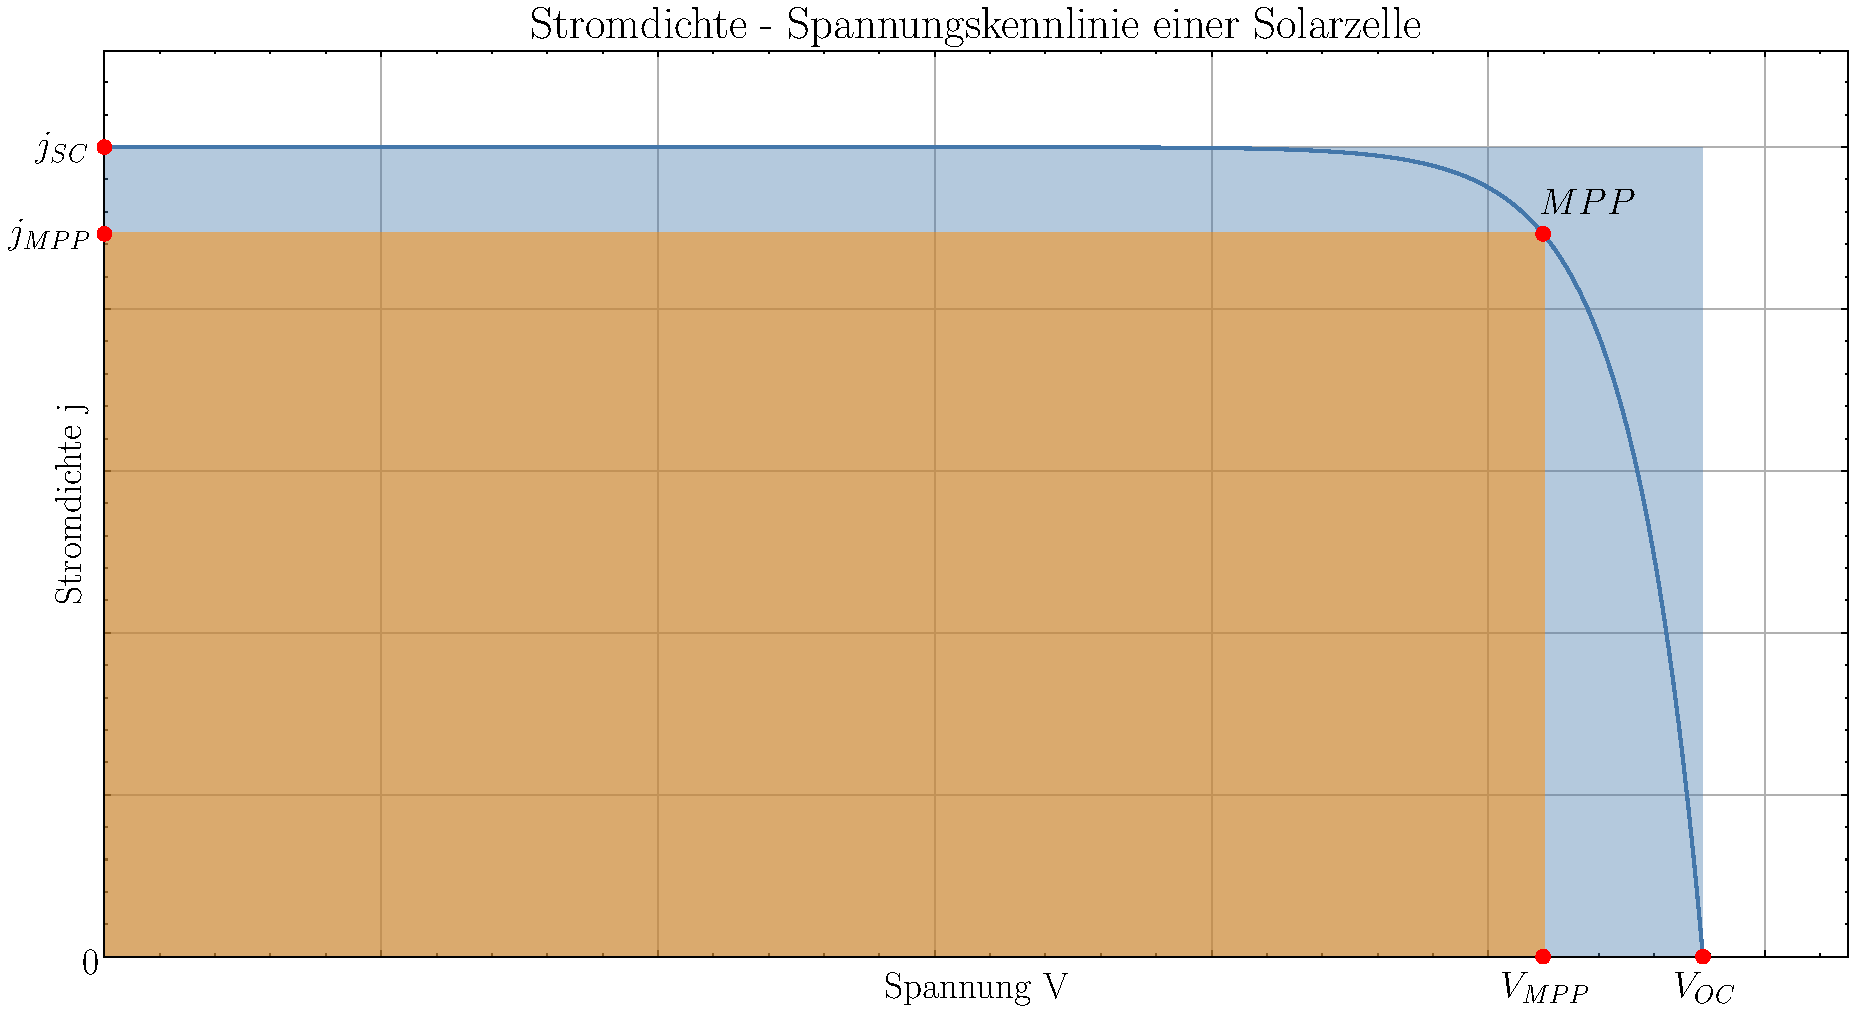
\includegraphics[width=\textwidth]{Bilder/SolarzelleIdeal.pdf}		
		\caption[Kennlinie ideale Solarzelle]{Stromdichte - Spannungskennlinie einer idealen Solarzelle, eingetragen sind zusätzlich wichtige Kenngrößen}
		\label{img:SolarzelleIdeal}
	\end{figure}
	Eine allgemeine Solarzelle verhält sich elektronisch ähnlich, wie eine Halbleiterdiode. In Abbildung \ref{img:SolarzelleIdeal} ist eine Solarzellenkennlinie abgebildet, der Unterschied zur Diodenkennlinie liegt allein in der Verschiebung in y-Richtung durch den Wert des Photostroms $j_{ph}$. Aus diesem Grund ist auch die Formel für die Stromcharakteristik bis auf diesen Wert identisch:
	\begin{equation}\label{eq:kennlinie}
		j(V) =  j_S \left(\text{exp}\left(\frac{e V}{m k_B T}\right) - 1\right) - j_{ph}
	\end{equation} 
	Der Photostrom kann für Perowskitsolarzellen folgendermaßen ausformuliert werden:
	\begin{equation}
		j_{ph} = e I_0 \eta_{CC} \eta_{inj} (1-\text{exp}(-\alpha d))
	\end{equation}
	Die dabei bisher aufgetretenen Variablen sind:
	\begin{itemize}
		\item Spannung $V$
		\item Sättigungsstromdichte $j_S$
		\item Elementarladung $e$ und Boltzmannkonstante $k_B$
		\item Idealitätsfaktor $m$
		\item Temperatur $T$
		\item Intensität des einfallenden Lichts $I_0$
		\item Effizienz für erzeugte Löcher/Elektronen transportierende Schichten zu erreichen $\eta_{CC}$
		\item Effizienz für Löcher/Elektronen in die Schichten einzutreten $\eta_{inj}$
		\item Absorptionskoeffizient $\alpha$
		\item Dicke der absorbierenden Schicht $d$
	\end{itemize}
	Nach dieser kurzen Einführung können die typischen Kenngrößen von Solarzellen erläutert werden.

	\paragraph{Kurzschlussstromdichte $j_{SC}$}
	Die Kurzschlussstromdichte ist gerade die Stromdichte bei einer Spannung von \SI{0}{\volt}, bei Belichtung einer Solarzelle. Sie ist in Abbildung \ref{img:SolarzelleIdeal} eingetragen, und entspricht dem Schnittpunkt mit der y-Achse der Kennlinie. Deshalb lässt sie sich folgend berechnen:
	\begin{equation}
		j_{SC} = j(V = 0) = e I_0 \eta_{CC} \eta_{inj} (1-\text{exp}(-\alpha d)) = j_{ph}
	\end{equation}
	\paragraph{Leerlaufspannung $V_{OC}$}
	Die Leerlaufspannung ist die Spannung bei einem Strom von \SI{0}{\ampere}, sie ist daher im Kennlinienfeld \ref{img:SolarzelleIdeal} als Nullstelle zu finden. Sie kann erneut aus der Gleichung \ref{eq:kennlinie} bestimmt werden:
	\begin{equation}
		\begin{split}
			 0 \overset{!}{=}  j_S \left(\text{exp}\left(\frac{e V_{OC}}{m k_B T}\right) - 1\right) - j_{ph}  \\
			 j_{ph} = j_S \, \text{exp}\left(\frac{e V_{OC}}{m k_B T}\right) \\
			 \Rightarrow V_{OC} = \text{ln} \left( \frac{j_{ph}}{j_S}\right) \frac{m k_B T}{e}
		\end{split}
	\end{equation} 
	Dabei wurde angenommen, dass $\text{exp}\left(\frac{e V_{OC}}{m k_B T}\right) \gg 1 $ und die Sättigungsstromdichte $j_{SC}$ entspricht gerade der Kurzschlussstromdichte $j_{SC}$, wie im Abschnitt davor gezeigt.
	\paragraph{Wirkungsgrad $\eta$}
	In der Abbildung \ref{img:SolarzelleIdeal} ist der sogenannte Maximum Power Point (MPP) eingetragen, er ist dort definiert, wo das Produkt aus der Stromdichte $j$ und der Spannung $V$ maximal ist. Die orangefarbene Fläche mit diesem Punkte, ist die maximale Leistungsdichte. Der Wirkungsgrad ist daher, dass Verhältnis aus dieser maximalen Leistungsdichte zur Leistungsdichte des eingestrahlten Lichts:
	\begin{equation}
		\eta = \frac{p_{max}}{p_0} = \frac{V_{MPP} \cdot j_{MPP}}{p_0}
	\end{equation}
	\paragraph{Füllfaktor FF}
	Aus den bisher beschriebenen Kenngrößen, kann der Füllfaktor angegeben werden, in der Abbildung .\ref{img:SolarzelleIdeal} ist eher das Verhältnis des orangen Rechtecks zum blauen Rechteck. Dieser Faktor gibt demnach das Verhältnis der Maximalleistung zur Leerlaufleistung an:
	\begin{equation}
		FF = \frac{V_{MPP} \cdot j_{MPP}}{V_{OC} \cdot j_{SC}}
	\end{equation}  

	\section{Aufbau einer Perowskitsolarzelle}
		\begin{figure}[ht]
		\centering
		\includegraphics[width=\textwidth]{Bilder/AufbauZelle.pdf}		
		\caption[Aufbau der Perowskit-Solarzelle]{Schematischer Aufbau der Perowskit-Solarzelle}
		\label{img:AufbauZelle}
	\end{figure}
	In Abbildung \ref{img:AufbauZelle} ist schematisch der schichtweise Aufbau einer Perowskit-Solarzelle abgebildet. Die einzelnen Schichten werden folgend von unten nach oben erläutert:
	\paragraph{Substrat}
	Die Solarzelle wird nach der Abbildung von der Unterseite beleuchtet, deshalb müssen die ersten Schichten transparent sein. Die erste Glas Schicht bildet eine stabile Unteralge für den Aufbau, dabei ist das Glas mit einem transparenten und leitfähigem Oxid beschichtet. zum Beispiel wird Fluordotiertes Zinnoxid (FTO) verwendet, dieses transportiert die entstehende Ladung zu einer Elektrode.
	\paragraph{n-leitende Schicht}
	Es folgt eine n-leitende Schicht, sie muss ebenfalls transparent sein und transportiert die in der Perowskitschicht entstehenden Elektronen ab. Häufige Verwendung findet hier Titanoxid \ce{TiO_{2}}.
	\paragraph{Perowskitschicht}
	In der Perowskitschicht werden Elektronen durch einstrahlende Photonen in das Valenzband gehoben, deshalb ist wichtig, dass diese Schicht einen hohen Absorptionskoeffizienten besitzt. In diesem Versuch wird Methylammoniumbleiiodid \ce{CH_3NH_3PbI_3} verwendet
		



	

\chapter{Aufbau und Durchführung}
	\fehlt
	
	


\chapter{Auswertung}
	\fehlt
\chapter{Fazit}
	\fehlt

\listoffigures%\addcontentsline{toc}{chapter}{\listfigurename}
	
\begin{thebibliography}{111}%\addcontentsline{toc}{chapter}{Literaturverzeichnis}
	\bibitem{Anleitung}
	Anleitung zum Fortgeschrittenen"~Praktikum.\\ \glqq Versuch: Organisch"~anorganisch hybride Perowskitsolarzellen\grqq.\\ Justus-Liebig-Universität Gießen. Sommersemester 2024.
	
	\bibitem{Perowskit}
		\fehlt
	\end{thebibliography}


\chapter*{Anhang}\label{ch:Anhang}\addcontentsline{toc}{chapter}{Anhang}
\FloatBarrier
	\begin{figure}[ht]
	\centering
%	\includegraphics[width=\textwidth]{data/Testat.pdf}		
	\caption[Testat]{Das Testat des Versuchs}
	\label{fig:Testat}
\end{figure}

\end{document}
